Sure, here's a more streamlined version of your text:

\subsection{Word Guessing Problem}
\label{sec:keen:operators:word_guessing}
  The \emph{Word Guessing Problem} (WGP) serves as a foundational illustration 
  of the implementation of genetic operators.
  At its core, the problem poses this challenge: evolve a population of strings
  to match a predefined target word.
  The metric of success or \enquote{fitness} for each individual string in this 
  population is measured by the number of its characters that align with the 
  target word.

  We will put these operators to the test against a range of target words, each 
  randomly generated and of varying lengths, ranging from 1 to 100 characters.

  Delving into the details:
  \begin{enumerate*}[label=(\roman*)]
    \item each gene in this context represents a non-nullable 16-bit Unicode 
      character, and
    \item the search space, given the constraints, can be formulated as:
  \end{enumerate*}
    
    \begin{equation}
    \label{eq:keen:operators:word_guessing:search_space}
      |S_\mathrm{WGP}| = (2^{16} - 1)^n = 65\,535^n
    \end{equation}

    Here, \(n\) denotes the length of the target word.

  The cardinality of the search space, presented on a logarithmic scale, can be 
  observed in \vref{fig:keen:operators:word_guessing:search_space}.

  \begin{figure}[ht!]
    \centering
    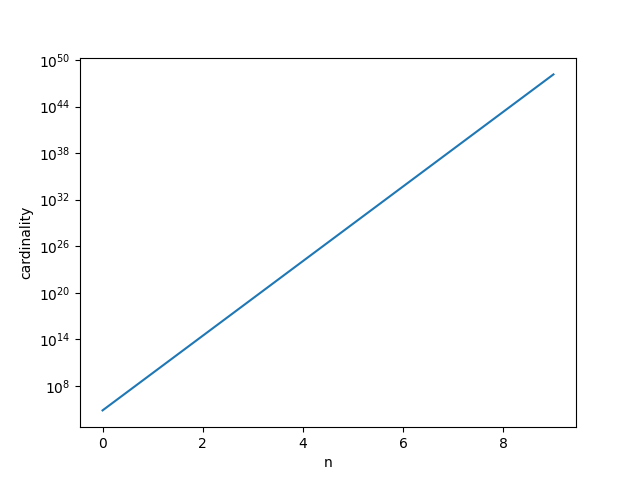
\includegraphics[width=0.6\textwidth]{img/keen/wgp_cardinality.png}
    \caption{Search space cardinality for the WGP on a logarithmic scale.}
    \label{fig:keen:operators:word_guessing:search_space}
  \end{figure}

  The evident exponential growth of the search space in relation to the length 
  of the target word emphasizes the impracticality of any exhaustive search 
  strategies.

  For the WGP, the fitness function remains straightforward.
  It necessitates a simple character comparison between the target word and the 
  individual string:

  \begin{equation}
  \label{eq:keen:operators:word_guessing:fitness}
    \phi_\mathrm{WGP}(i) = \sum_{j=0}^{n-1} \delta(i_j, t_j)
  \end{equation}

  Here, \(i\) represents the individual string, \(t\) stands for the target 
  word, \(n\) specifies the target word's length, and \(\delta\) is the 
  \textit{Kronecker delta function}, further detailed in \vref{def:kronecker}.
